\documentclass[12pt,a4paper]{article}
\usepackage[utf8]{inputenc}
\usepackage[portuguese]{babel}
\usepackage{graphicx}
\usepackage{cite}
\usepackage{hyperref}
\usepackage{times}
\usepackage[top=3.5cm, bottom=2.5cm, left=3.0cm, right=3.0cm]{geometry}
\usepackage{amsmath}
\usepackage{caption}
\captionsetup{font={sf,bf,footnotesize}}

\pagestyle{empty}

\renewenvironment{abstract}
  {\list{}{\setlength{\leftmargin}{0.8cm}\setlength{\rightmargin}{0.8cm}\fontsize{12}{14}\selectfont}\item\relax}
  {\endlist}

\title{\textbf{Análise de Desempenho e Consumo de Memória dos Algoritmos Quick Sort, Heap Sort e Radix Sort em Python}}
\author{\textbf{Felippe Henrique Teixeira Pedroso}\\
Universidade Tecnológica Federal do Paraná\\
{\tt \small felippepedroso@alunos.utfpr.edu.br}}
\date{}

\begin{document}
\maketitle
\thispagestyle{empty}

\begin{abstract}
\noindent \textbf{Resumo.} 
A ordenação de dados é uma das operações mais fundamentais dos sistemas de informação, podendo ser realizada de inúmeras formas. O propósito deste estudo é analisar comparativamente as variáveis de performance de três algoritmos: Quick Sort, Heap Sort e Radix Sort. O código foi escrito na linguagem Python, utilizando vetores com tamanhos variando de 1.000 a 20.000 elementos, tanto desordenados aleatoriamente quanto ordenados inversamente, coletando-se as métricas de tempo, comparações, trocas e memória para cada caso. A conclusão principal foi a eficiência de métodos não-comparativos, como o Radix Sort, contraposta com seu maior uso de memória, e a performance mais equilibrada de algoritmos \textit{in-place} comparativos, como o Quick Sort.
\end{abstract}

\vspace{0.4cm}

\begin{abstract}
\noindent \textbf{Abstract.}
Data sorting is one of the most fundamental operations in information systems and can be performed in numerous ways. The purpose of this study is to perform a comparative analysis of the performance variables of three algorithms: Quick Sort, Heap Sort, and Radix Sort. The code was written in Python, using array sizes ranging from 1,000 to 20,000 elements, across both randomly shuffled and inversely ordered distributions, collecting metrics for execution time, comparisons, swaps, and memory usage for each case. The main conclusion highlighted the efficiency of non-comparative methods, such as Radix Sort, contrasted with their higher memory consumption, and the more balanced performance of comparative \textit{in-place} algorithms, such as Quick Sort.
\end{abstract}

\section{Introdução}
\subsection{Contextualização}
Quando se trata das operações mais utilizadas e necessárias na computação, a ordenação de dados se destaca não somente por si mesma, mas também como sub-rotina de vários algoritmos mais complexos, sendo uma peça integral para diversas áreas no grande escopo do gerenciamento de dados. Sendo assim, a escolha do método de ordenação, dentre as centenas já criados, deve ser analisada além da simples quantidade expressa de elementos $n$ a serem ordenados, considerando também o ambiente de \textit{software} e \textit{hardware} utilizado, o estado inicial dos dados e o caso de uso específico. Logo, é possível afirmar que nenhum algoritmo de ordenação é absolutamente superior em todos os cenários possíveis de aplicação \cite{cormen2012}.

Nesse interesse, é importante entender as classificações e características individuais de cada algoritmo e, portanto, como elas afetam seus casos de uso. Entre elas, a distinção entre métodos comparativos e não-comparativos é uma das divisões primárias a serem feitas, dado que representa o fundamento da interação entre o algoritmo e seus dados. Técnicas de ordenação baseadas unicamente em comparações irão requerer no mínimo $\sim n \log_2 n$ operações em seus piores casos, sendo esse limite superado principalmente ao se utilizar informações internas das chaves, como seus dígitos ou bits. Já métodos não-comparativos oferecem um limiar maior de eficiência; porém, cobram na otimização do espaço, podendo exigir diversos arranjos e estruturas de dados auxiliares proporcionais a $n$. Isso os difere dos algoritmos \textit{in-place}, que realizam todas as suas operações dentro do armazenamento original das informações \cite{sedgewick2011}.

\subsection{Objetivo do Trabalho}
O propósito deste trabalho é realizar uma análise empírica em Python comparando três algoritmos de ordenação: Quick Sort, Heap Sort e Radix Sort. Para isso, foram definidos quatro tamanhos de vetores de entrada e duas situações iniciais para cada, totalizando dezesseis cenários únicos de ordenação. As dimensões utilizadas foram de 1.000, 5.000, 10.000 e 20.000 elementos, divididas para situações de ordenação aleatória e inversa (números decrescentes). As métricas de comparação utilizadas em cada cenário foram: o tempo de execução em milissegundos, o consumo de RAM em MB (megabytes), a quantidade de trocas e a de comparações.

A fundamentação teórica dos três algoritmos pode ser encontrada na Seção 2, onde as complexidades e particularidades de cada um foram destacadas e cruzadas com seu caso típico de uso. Na Seção 3, a metodologia experimental e as especificações do ambiente de \textit{hardware} e \textit{software} foram detalhadas a fim de posicionar os resultados de forma contextualmente correta. Já a Seção 4 analisa e discute os resultados empíricos obtidos, fornecendo gráficos e observações decorrentes das informações coletadas. Por fim, a Seção 5 expõe as conclusões e considerações finais do estudo e suas consequências.

\section{Fundamentação Teórica}

\subsection{Quick Sort}
O método proposto por C. A. R. Hoare em 1960 emprega a técnica conhecida como Divisão e Conquista. Seu funcionamento se baseia na escolha de um elemento-pivô, que é utilizado como base para o particionamento e a reorganização do vetor de dados. Este é dividido em dois sub-arranjos a partir do pivô, os quais são ordenados e resultam em uma lista com todos os elementos menores que o pivô à esquerda e todos os maiores à direita. A escolha de qual elemento será o pivô é um dos gargalos mais conhecidos do método; por isso, a utilização do \textit{Randomized Quick Sort}, nome derivado da seleção aleatória do pivô, é uma abordagem clássica para evitar a degradação de desempenho que ocorre em particionamentos determinísticos de vetores pré-ordenados \cite{cormen2012}.

O caso médio assintótico, assim como o melhor caso da versão otimizada supracitada, possui complexidade garantida em $O(n \log n)$ com alta probabilidade, mantendo o consumo de memória restrito às chamadas recursivas. Isto se deve ao fato de suas operações serem feitas \textit{in-place}, ou seja, na mesma estrutura de dados originalmente repassada para o algoritmo, permitindo que sua necessidade de memória auxiliar seja restrita ao tamanho da pilha de recursão, descrita por $O(\log n)$. 
Já seu pior caso, considerando a escolha do pior pivô em um vetor ordenado inversamente (o que implica maior quantidade de trocas para organizar os elementos em relação ao pivô), é denotado por $O(n^2)$. Todavia, sua alta velocidade e baixo uso de memória são aspectos que rendem a esse algoritmo a reputação de ser um dos métodos mais rápidos e versáteis, principalmente para grandes conjuntos de dados \cite{sedgewick2011}.

\subsection{Heap Sort}
Para entender o Heap Sort, é essencial compreender o conceito de Max-Heap. Esta é uma estrutura ``planificada'' de uma árvore binária quase completa, organizada dentro de um vetor unidimensional, onde cada nó pai é sempre maior ou igual aos seus nós filhos. Nessa representação, cada nó $i$ possui dois filhos situados nos índices $2i + 1$ e $2i + 2$, enquanto o pai de qualquer nó filho (excluindo a raiz) é localizado pelo índice $\lfloor (i - 1)/2 \rfloor$. O Heap Sort atua como um meio-termo entre métodos simples e avançados, combinando a eficiência de tempo de algoritmos de Divisão e Conquista, como o Merge Sort, com a economia de espaço de algoritmos \textit{in-place}, como o Insertion Sort \cite{cormen2012}.

O algoritmo se baseia em organizar inicialmente o vetor sob a definição de uma Max-Heap, processo conhecido como construção do heap (\textit{build-max-heap}), executado em tempo linear $O(n)$. Após essa estruturação inicial, o algoritmo extrai a raiz e a posiciona no último índice não ordenado do vetor, dado que, por definição, ela contém o maior elemento. Em seguida, é necessário restabelecer a propriedade de Max-Heap no sub-arranjo restante (\textit{heapify}), ajuste que consome tempo $O(\log n)$ a cada remoção. Essas propriedades conferem ao Heap Sort o destaque teórico de garantir estritamente um tempo de execução $O(n \log n)$ em todos os cenários (pior, médio e melhor caso), combinada a um consumo de memória auxiliar constante $O(1)$ \cite{sedgewick2011}.

\subsection{Radix Sort}
Ademais, o Radix Sort se destaca como um exemplo indispensável de método não-compa-rativo, baseando-se na utilização de estruturas de memória tratadas de forma especializada para realizar as ordenações. Essa característica permite a ele romper o limite teórico inferior de $\Omega(n \log n)$, já que não realiza comparações relativas de magnitude entre as chaves, processando diretamente a estrutura interna dos elementos (seus dígitos ou bits). Sendo assim, uma de suas abordagens mais eficientes é a \textit{Least Significant Digit} (LSD), na qual a ordenação começa nos algarismos de menor valor posicional e progride para os de maior valor, utilizando estruturas de memória chamadas \textit{buckets} para reorganizar os dados \cite{cormen2012}.

No entanto, esse estilo de abordagem exige atenção à estabilidade para não alterar a posição de elementos com dígitos de mesmo valor. A resolução desse problema é feita utilizando uma sub-rotina estritamente estável, geralmente o Counting Sort (rotina padrão para essa função, pois utiliza a contagem de frequências e somas dos dígitos), preservando a ordem relativa dos dígitos idênticos. Essa lógica resulta em uma complexidade total em tempo linear $O(n \cdot k)$, em que $k$ é o número máximo de dígitos por chave. Contudo, esse ganho em velocidade cobra um preço na memória: a necessidade de vetores auxiliares para a contagem e saída exige complexidade $O(n + k)$, o que significa que o algoritmo não é \textit{in-place} e consome mais RAM que métodos puramente comparativos \cite{sedgewick2011}.

\section{Metodologia Experimental}
\subsection{Cenários de Teste}
O primeiro cenário utilizado consistiu em listas desordenadas aleatoriamente, criadas a partir da geração uniforme de números inteiros randômicos não repetidos. Esse caso busca simular entradas comuns e avaliar o caso médio. O outro caso testado foi o de listas ordenadas de forma decrescente, partindo de $n$ até $0$; isso tem o propósito de se aproximar do pior caso para a maioria dos algoritmos. Para mitigar a instabilidade de \textit{software} e \textit{hardware}, cada cenário foi executado cinco vezes (considerando também o tamanho de entrada por caso), adotando-se as médias aritméticas de todas as métricas para obter resultados experimentalmente mais válidos.

\subsection{Tamanhos de Entrada}
Os volumes de dados avaliados foram de 1.000, 5.000, 10.000 e 20.000 elementos, ou seja, $N \in \{1.000, 5.000, 10.000, 20.000\}$. Com base nisso, estabeleceu-se uma matriz de teste com 24 combinações únicas ($3 \text{ algoritmos} \times 4 \text{ tamanhos} \times 2 \text{ distribuições}$). Considerando as execuções repetidas para extração das médias, realizaram-se 120 execuções individuais para preencher o \textit{benchmark} com os dados empíricos. Essa amostra demonstrou-se suficiente nos ambientes selecionados para a aferição relativa de performance.

\subsection{Métricas de Avaliação}
A primeira métrica, e geralmente a mais importante, foi o tempo de execução. Ele foi capturado em milissegundos utilizando funções de alta precisão presentes na linguagem de programação adotada. A segunda foi o consumo de memória RAM em MB (megabytes), monitorando-se os picos de alocação extra para medir de forma precisa o seu uso e permitir a observação clara do impacto dos paradigmas comparativos e não-comparativos. A terceira métrica foi a quantidade de comparações feitas dentro do ciclo inteiro do algoritmo, variável também essencial para visualizar as propriedades teóricas dos métodos. A quarta e última métrica foi o número de trocas, ou seja, quantas vezes foi necessário realizar um deslocamento de dados dentro do ciclo completo de ordenação.

\subsection{Ambiente de Hardware e Software}
A linguagem utilizada foi Python 3.13, com todo o código-fonte e scripts de benchmark disponibilizados publicamente em repositório no GitHub\footnote{\url{https://github.com/felippehtp/Sorting-Algorithms-ED2}} sobre o sistema operacional Windows 11. Foram utilizadas as bibliotecas \textit{pandas} para estruturação dos dados e \textit{matplotlib} em conjunto com \textit{seaborn} para a síntese dos gráficos. As especificações do dispositivo utilizado nos testes são: um processador AMD Ryzen 5 5500 de 3.6 GHz e uma memória RAM de 16 GB com $\sim$2.666 MT/s de velocidade.

\section{Resultados e Discussão}

\begin{figure}[htbp]
  \centering
  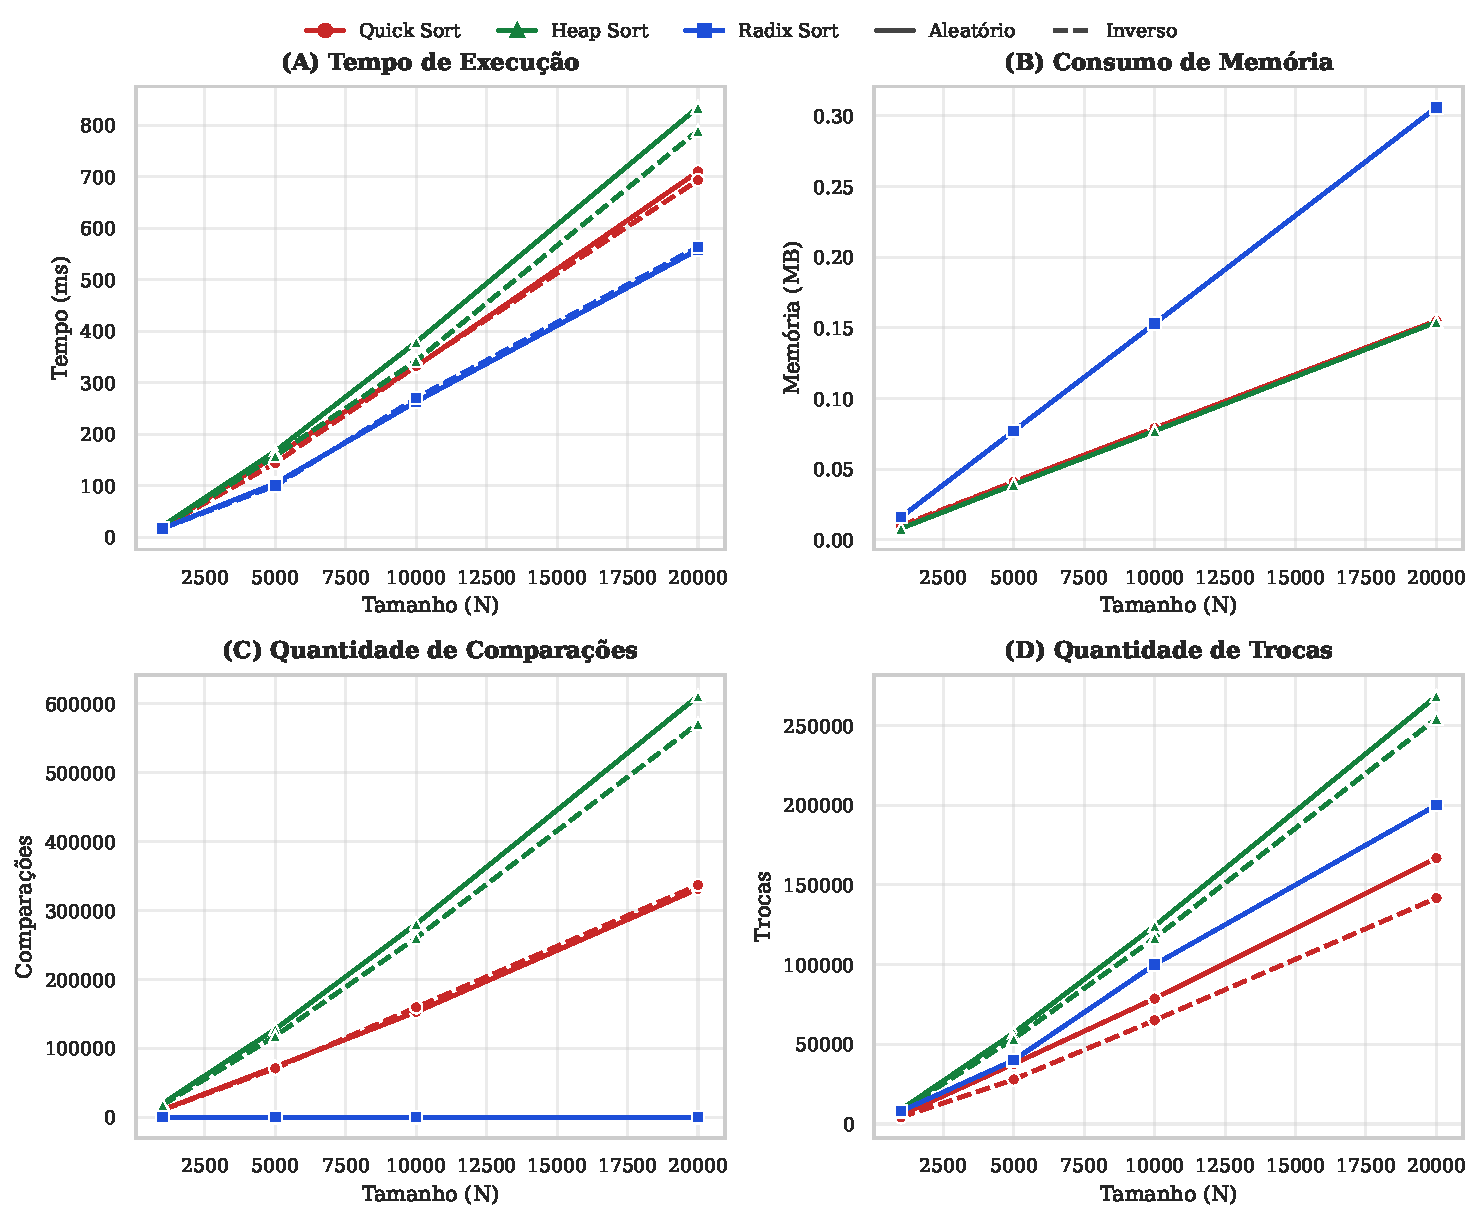
\includegraphics[width=0.98\textwidth]{graficos_desempenho.pdf}
\caption{Análise comparativa de desempenho entre os algoritmos Quick Sort, Heap Sort e Radix Sort para as métricas de (A) Tempo de Execução, (B) Consumo de Memória, (C) Quantidade de Comparações e (D) Quantidade de Trocas.}
  \label{fig:desempenho}
\end{figure}

A Figura \ref{fig:desempenho} sintetiza os dados empíricos coletados ao longo do experimento, permitindo analisar o comportamento dos três algoritmos frente às variações de tamanho de entrada e de distribuição dos dados.

\subsection{Desempenho em Listas Aleatórias}
No cenário de entradas desordenadas aleatoriamente, o Radix Sort obteve o menor tempo de execução para todas as dimensões testadas, atingindo $558{,}37\text{ ms}$ no tamanho máximo de $20.000$ elementos; essa vantagem teórica e prática decorre de sua complexidade linear-aritmética $O(n \cdot k)$, que rompe a barreira de $\Omega(n \log n)$ dos algoritmos comparativos. O Quick Sort registrou o segundo melhor tempo de execução, alcançando $709{,}98\text{ ms}$ em $N = 20.000$, superando o Heap Sort, que finalizou com $834{,}71\text{ ms}$. Quanto ao uso de memória RAM, Quick Sort e Heap Sort mantiveram um consumo idêntico e reduzido de $0{,}15\text{ MB}$ para $20.000$ elementos, confirmando a característica \textit{in-place}; já o Radix Sort demandou o dobro de memória ($0{,}30\text{ MB}$) devido à alocação de vetores auxiliares para a execução do Counting Sort. Por fim, o Radix Sort não realizou comparações em nenhum momento, enquanto o Quick Sort efetuou menos comparações ($331.467$) e trocas ($166.780$) do que o Heap Sort ($611.232$ comparações e $268.387$ trocas).

\subsection{Desempenho em Listas Inversas}
No cenário de vetores ordenados inversamente, os algoritmos comparativos apresentaram um desempenho ligeiramente superior se comparado ao cenário aleatório, o que pode parecer contraintuitivo à primeira vista, dado que vetores decrescentes costumam ser associados ao pior caso teórico. No entanto, o tempo do Quick Sort reduziu para $693{,}36\text{ ms}$ e o do Heap Sort caiu para $789{,}51\text{ ms}$ em $N = 20.000$. Esse ganho de performance está diretamente ligado à redução do número de trocas: no Quick Sort, o total de trocas caiu para $141.735$, pois a disposição monotônica decrescente dos elementos reduz os deslocamentos necessários na partição ao redor do pivô sorteado; no Heap Sort, as trocas caíram para $254.334$, dado que o maior elemento já se encontra na primeira posição do vetor, agilizando a fase de construção inicial da Max-Heap. Ademais, a ordenação estrita dos dados favorece a predição de desvios (\textit{branch prediction}) do processador, minimizando travamentos no fluxo de execução de instruções da CPU.

\subsection{Análise Comparativa}
Os dados coletados evidenciam o \textit{trade-off} clássico entre tempo de processamento e uso de memória RAM. Embora o Radix Sort seja o método mais rápido entre os testados, sua natureza \textit{out-of-place} cobra um custo extra no consumo de memória. Já entre os métodos comparativos \textit{in-place}, a superioridade em tempo do Quick Sort em relação ao Heap Sort, mesmo ambos compartilhando a mesma complexidade assintótica $O(n \log n)$, se deve à maior localidade de referência (\textit{cache locality}) no particionamento contínuo da memória. Essa característica minimiza falhas de \textit{cache} (\textit{cache misses}) quando comparada aos saltos de índice típicos da estrutura de árvore do Heap Sort \cite{sedgewick2011}.

\section{Conclusão}
Este trabalho realizou uma análise comparativa empírica entre os algoritmos Quick Sort, Heap Sort e Radix Sort, avaliando as métricas de tempo, memória, comparações e trocas em quatro tamanhos de entrada ($1.000$ a $20.000$ elementos) sob distribuições aleatórias e inversas. A utilização da média de cinco execuções consecutivas por cenário permitiu mitigar oscilações do ambiente de testes e obter dados experimentalmente válidos.

Com isso, conclui-se que o Radix Sort representa a escolha ideal em termos de velocidade temporal quando há disponibilidade de memória RAM no sistema. Para ambientes com restrição estrita de memória, o Quick Sort consolida-se como o algoritmo de uso geral mais equilibrado, combinando a propriedade \textit{in-place} com tempos de execução reduzidos. Por fim, o Heap Sort atua como uma solução segura por garantir limites rígidos de desempenho sem risco de degradação. Como trabalhos futuros, sugere-se a ampliação dos testes para conjuntos de dados superiores a $10^6$ elementos e a avaliação com tipos de dados heterogêneos.

\begin{thebibliography}{9}

\bibitem{cormen2012}
T. H. Cormen, C. E. Leiserson, R. L. Rivest, and C. Stein, \textit{Algoritmos: teoria e prática}, 3rd ed. Rio de Janeiro: Elsevier, 2012.

\bibitem{sedgewick2011}
R. Sedgewick and K. Wayne, \textit{Algorithms}, 4th ed. Boston: Addison-Wesley, 2011.

\end{thebibliography}

\end{document}